\documentclass[lang=cn,10pt]{elegantbook}
\usepackage{subcaption}


\newcommand\bv[1]{\boldsymbol{#1}}
\newcommand\mb[1]{\mathbb{#1}}
\newcommand\mc[1]{\mathcal{#1}}

% \title{Complex Analysis}
% \subtitle{Elegant\LaTeX{} 经典之作}

\author{Lollins}
% \institute{Elegant\LaTeX{} Program}
\date{\today}
% \version{4.3}
% \bioinfo{自定义}{信息}

\extrainfo{改变人生的事情,你必须冒险;
	意义非凡的事情,大多碰巧发生;
	不重要的事,才有周全的计划。
}

\setcounter{tocdepth}{2}

\logo{logo1.jpg}
\cover{cover.jpg}

% 本文档命令
\usepackage{array}
\newcommand{\ccr}[1]{\makecell{{\color{#1}\rule{1cm}{1cm}}}}

% 修改标题页的橙色带
% \definecolor{customcolor}{RGB}{32,178,170}
% \colorlet{coverlinecolor}{customcolor}

\begin{document}

\title{非参数统计分析}
\author{Lollins}
\date{\today}

\maketitle

\pagenumbering{roman}
\setcounter{page}{1}

\begin{center}
    \Huge\textbf{前言}
\end{center}
\par
非参数统计分析笔记,一些图片的代码在code文件夹下。


\begin{flushright}
    \begin{tabular}{c}
        Lollins \\
        \today
    \end{tabular}
\end{flushright}

\newpage
\pagenumbering{Roman}
\setcounter{page}{1}
\tableofcontents
\newpage
\setcounter{page}{1}
\pagenumbering{arabic}

\chapter{绪论}
\section{序}
\subsection{非参数统计概念及学习意义}
\subsubsection{意义}
\subsubsection{概念}
\begin{itemize}
    \item \textbf{参数统计方法:}数据样本被视为从分布族的某个参数族抽取出来的总体的代表,
          未知的仅仅是总体分布具体数值,这样推断问题就转化为分布族的若干未知参数的估计问题,
          用样本来对这些参数进行估计或进行假设检验,从而得知背后的分布,这类推断方法称为参数
          统计方法。
    \item \textbf{非参数统计方法:}不假定总体分布的具体形式,尽量从数据(或样本)本身获得所需要的信息,
          通过估计而获得分布的结构,并逐步建立对事物的数学描述和统计模型的方法。
\end{itemize}

\subsection{非参数统计的历史及发展}

\section{引言}
\subsection{参数统计方法与非参数统计方法的区别}
\begin{itemize}
    \item \textbf{参数统计方法:}假定总体的分布形式,既利用样本的数据信息,又利用产生数据总体的信息,是一个有效的数据
          分析方法,针对性强,但可能出现大的错误。
    \item \textbf{非参数统计方法:}不假定总体的分布形式,更接近大多数实际情况,故不会出现大的错误。
\end{itemize}

\subsection{非参数统计方法的特点}

\begin{enumerate}[(1)]
    \item 有广泛的适用性(广)
    \item 样本方法是非参数统计的基本方法(样本)
    \item 计算简单(简)
    \item 良好的稳定性(稳)
\end{enumerate}

\chapter{描述性统计}
\begin{definition}[描述性统计]
    是在对产生数据的总体的分布不作任何假设的情况下,整理数据、
    显示数据、分析数据,将数据中有用的信息提取出来的统计方法。
    本章介绍常用的描述性统计方法:\textbf{表格法、图形法和数值方法}。
\end{definition}

\section{图表法}
表格法、图形法描述统计数据主要是频数(率)分布表和直方图。

\section{数值方法}
数值方法主要是用数值来表示数据的中心位置和离散程度等的方法。

\subsection{表示中心位置的数值}
我们要求数据的中心位置满足这样一个\textbf{条件:}它到各个数据点的距离的和比较小。
表示中心位置的数值有平均数、中位数、众数、切尾平均数。

\subsubsection{平均数}
如果用平方值距离法,则点a到各数据点$x_1,x_2,...,x_n$的距离的和可以用
$\sum_{i=1}^{n}(x_i-a)^2$来衡量。平均数$\bar{x} = \frac{\sum_{i=1}^{n}x_i}{n}$满足条件:
\begin{equation}
    \sum_{i=1}^n\left(x_i-\bar{x}\right)^2=\min_a\sum_{i=1}^n\left(x_i-a\right)^2
\end{equation}
上式表示\textbf{平均数这一点到各个数据点的平方值距离和最短}。所以在\textbf{平方值距离方法下},数据中心位置的代表是\textbf{平均数}。

\subsubsection{中位数}
如果用绝对值距离法,则点a到各数据点$x_1,x_2,...,x_n$的距离的和可以用$\sum_{i=1}^{n}|x_i-a|$
来衡量,中位数me满足条件:
\begin{equation}
    \sum_{i=1}^n|x_i-\max|=\min_a\sum_{i=1}^n|x_i-a|
\end{equation}
上式表示\textbf{中位数这一点到各个数据点的绝对值距离和最短}。所以在\textbf{绝对值距离方法下},数据中心位置的代表是\textbf{中位数}。

\textbf{注:}
\begin{itemize}
    \item 中位数是非线性规划选址问题的解;
    \item 中位数不受极大(小)的影响,有时能较好地表示数据的中心位置。
\end{itemize}

\subsubsection{众数}
众数:一组数据中出现频数最高的数据。

\textbf{注:}
\begin{itemize}
    \item 众数也能描述数据的中心位置。特别是定性数据;
    \item 一组数据有偏时,若数据右偏(Positively Skewed),通常有$mo < me < \bar{x}$,
          若数据左偏(Negatively Skewed),通常有$\bar{x} < me < mo$,见图\ref{im2_1}。
\end{itemize}

\begin{figure}
    \centering
    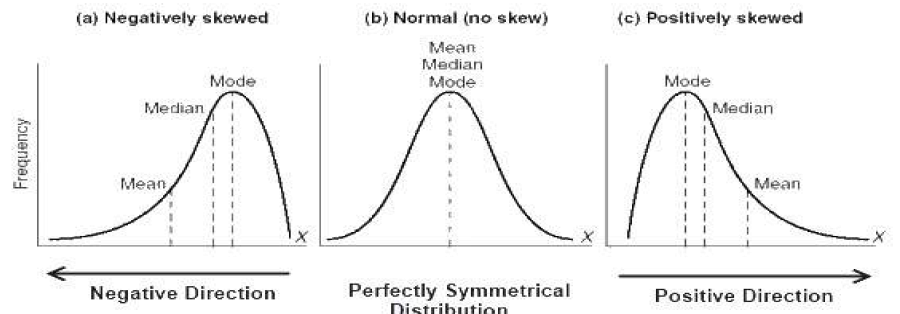
\includegraphics[scale = 0.6]{img/2_1.png}
    \caption{}
    \label{im2_1}
\end{figure}

\subsubsection{切尾平均数}
设$X_{(1)},...,X_{(n)}\text{是来自总体X的简单随机样本}X_{1},...,X_{n}$的次序统计值,称
\begin{equation}
    T_{nk}=\frac{1}{n-2k}(x_{(k+1)}+\ldots+x_{(n-k)})
\end{equation}
为原样本的的切尾均值。

\subsection{表示离散程度的数值}
样本方差、标准差、全距(范围)、四分位数间距。

\subsection{标准误}
\begin{equation}
    se = \frac{s}{\sqrt{n}},s\text{为样本标准差}
\end{equation}

\subsection{偏度}
偏度反映单峰分布对称性,常用$\beta_s$表示总体偏度,
\begin{equation}
    \beta_s=E[(\frac{x-\mu}\sigma)^3]=\frac{\mu_3}{\sigma^3},\text{其中}\mu_3=E(x-\mu)^3
\end{equation}

\textbf{注:}对称分布的偏度$\beta_s=0$;反之不成立,即$\beta_s=0$,不一定是对称分布。

样本偏度用$b_s$表示,
\begin{equation}
    b_s=\frac{m_3}{m_2^{\frac{3}{2}}},\text{其中}m_j=\frac{1}{n}\sum_i(x_i-\overline{x})^j
\end{equation}

\textbf{注:}$b_s>0$时,倾向于认为数据分布右偏;$b_s<0$时,倾向于认为数据分布左偏;
$b_s\approx 0$时,倾向认为数据分布是对称的。

\subsection{峰度}
峰度反映分布峰的尖峭程度,常用$\beta_k$表示总体峰度。
\begin{equation}
    \beta_k=E[(\frac{x-\mu}{\sigma})^4]=\frac{\mu_4}{\sigma^4}
\end{equation}

\textbf{注:}若$X\sim N(\mu,\sigma^2)$,则$\beta_k=3$。当$\beta_k>3$时,该分布具有过度的峰度(厚尾分布),
当$\beta_k<3$时,该分布具有不足的峰度(薄尾分布),

样本峰度用$b_k$表示,
\begin{equation}
    b_k=\frac{m_4}{(m_2)^2}
\end{equation}

\chapter{符号检验法}
在非参数检验中,总体的中心位置的数通常用中位数表示,本章主要讨论中位数、p分位数检验
问题的符号检验方法,中位数的点估计、区间估计等。
\section{符号检验}
\subsection{具体操作方法}
符号检验问题的原假设和备择假设有三种情况。这三种情况的原假设$H_0$都是$me = me_0$,其中$me_0$是给定的常数,
备择假设$H_1$分别是$me>me_0,me<me_0$和$me \ne me_0$。

由于$P(X=me)=0$,所以不妨假设样本单元$x_1,x_2,...,x_n$都不等于$me_0$。
符号检验的检验统计量为
\begin{equation}
    S^+ ={}^{\#}G= {}^{\#}\{x_i:x_i-\text{me}_0>0,i=1,2,\cdots,n\},
\end{equation}
记号\#表示计数,即$S^+$是集合$G$中元素的个数。$S^+$也可以等价的表示为
\begin{equation}
    S^+=\sum_{i=1}^nu_i,u_i=
    \begin{cases}
        1, & x_i-me_0>0   \\
        0, & \text{否则,}
    \end{cases},{\begin{array}{c}
                i=1,2,\cdots,n \\
            \end{array}}
\end{equation}
由于在$me = me_0$时,$S^+\sim b(n,\frac12)$。

考虑备择假设$H_1:me>me_0$,我们用$p$值来度量$S^+$是否足够大,让我们拒接原假设。
$p$值等于二项分布$b(n,\frac12)$的随机变量大于等于$S^+$的概率$P(b(n,\frac12)\geq S^+)$,
$p$值越小,$S^+$越大。

如果$p$值$\leq \alpha$,则在显著性水平$\alpha$下拒接原假设,认为备择假设$H_1$成立;
如果$p$值$> \alpha$,则在显著性水平$\alpha$下不拒绝原假设。

\subsection{注意事项}
在实际问题中,可能出现一些观察值正好等于$me_0$,这时有以下两种处理方法:
\begin{enumerate}[1、]
    \item 将这些正好等于$me_0$的观察值去掉,并相应的减少样本容量$n$的值。
    \item (不常用,不写了)
\end{enumerate}

\subsection{中位数的估计}
\subsubsection{点估计}
\begin{lemma}\label{le3.1}
    设$x_1,x_2,...,x_n$是来自总体X的样本,$t_p$为总体X的p分位数,$m_{np}$
    为样本的p分位数,则
    \begin{equation}
        P(\lim_{n \to \infty} m_{np} = t_p ) = 1
    \end{equation}
\end{lemma}
根据引理\ref{le3.1},我们可以结论
\begin{equation}
    \hat{t}_p = m_{np} = \begin{cases}
        x_{([np]+1)},                 & np\text{为非整数} \\
        \frac12(x_{(np+1)}+x_{(np)}), & np\text{为整数}
    \end{cases}
\end{equation}

\subsubsection{区间估计}
设$x_1,x_2,...,x_n$是来自总体X的样本,$S^+ =
    {}^{\#}\{x_i:x_i-\text{me}_0>0,i=1,2,\cdots,n\}\sim b(n,\frac12)$
那么有
\begin{equation}
    P(x_{(r)}\leq me \leq x_{(n-r+1)}) =1-P(me < x_{(r)}) -P(me > x_{(n-r+1)})
    = 1-\sum_{i=0}^{r-1}\binom{n}{i}(\frac{1}{2})^{n-1}
\end{equation}
\textbf{注:}层数r越大,置信区间越短,置信水平越低(置信水平为$1-\alpha$)。

\section{符号检验在定性数据分析中的应用}
根据中心极限定理,当n很大时,且$S^+ \sim b(n,p)$,那么$z=\frac{S^+ - np}{\sqrt{np(1-p)}}\sim N(0,1)$。

对于$x\sim b(n,p)$,做连续性修正:
\begin{enumerate}[1、]
    \item $P(X\leq k)\approx\Phi(\frac{k+\frac12-np}{\sqrt{np(1-p)}}),
              P(X< k)\approx\Phi(\frac{k-\frac12-np}{\sqrt{np(1-p)}})$
    \item $P(X\geq k)\approx\Phi(\frac{np-k+\frac12}{\sqrt{np(1-p)}}),
              P(X> k)\approx\Phi(\frac{np-k-\frac12}{\sqrt{np(1-p)}})$
\end{enumerate}

\section{成对数据的比较问题}
\begin{definition}[配对数据]
    两样本间配偶成对,每一对样本除随机给予的不同处理外,其他试验条件尽量一致。
\end{definition}

\chapter{符号秩和检验法}
本章主要讨论对称中心的检验及估计问题。
\section{对称中心为原点的检验问题}
\subsection{符号秩和检验统计量$W^+$}
\textbf{符号检验统计量}
\begin{equation}\label{eq4.1}
    S^+=\sum_{i=1}^nu_i,u_i=
    \begin{cases}1,\quad & x_i>0,       \\
             0,\quad & \text{否则,}
    \end{cases}i=1,2,\cdots,n.
\end{equation}
\textbf{注:}$S^+$仅使用样本数据量的正负信息,未使用样本数据量的大小信息。

\textbf{符号秩和统计量}

设$|x_1|,|x_2|,\cdots,|x_n|$互不相等,由大到小排列为$z_{(1)}<z_{(2)}<\cdots<z_{(n)}$,
若$|x_i|=z_{(R_i)}$,则称$|x_i|$的秩为$R_i,R_{i}=1,2,\cdots,n$。符号秩和统计量为
\begin{equation}
    W^+=\sum_{i=1}^nu_iR_i
\end{equation}
此处的$u_i$定义与式\ref{eq4.1}中相同。

\textbf{注:}$W^+$不仅使用样本数据量的符号信息,还是使用了样本数据量的大小信息。

在表\ref{ta4.1}中给出了10个观察值以及它们的10个观察值的符号,绝对值和绝对值的秩。
\begin{table}[htbp]
    \centering
    \caption{10个观察值的符号,绝对值和绝对值的秩}
    \label{ta4.1}
    \begin{tabular}{c|c|c|c|c|c|c|c|c|c|c}
        \hline
        观察值     & -7.6 & -5.5 & 4.3 & 2.7 & -4.8 & 2.1 & -1.2 & -6.6 & -3.3 & -8.5 \\
        \hline
        符号       & -    & -    & +   & +   & -    & +   & -    & -    & -    & -    \\
        \hline
        绝对值     & 7.6  & 5.5  & 4.3 & 2.7 & 4.8  & 2.1 & 1.2  & 6.6  & 3.3  & 8.5  \\
        \hline
        绝对值的秩 & 9    & 7    & 5   & 3   & 6    & 2   & 1    & 8    & 4    & 10   \\
        \hline
    \end{tabular}
\end{table}
这10个观察值的符号检验统计量$S^+=3$,符号秩和统计量$W^+=5+3+2=10$。

\subsection{符号秩和检验}
检验统计量:$W^+$,原假设$H_0:\theta = 0$

1、备择假设$H_1:\theta>0$,
若备择假设$H_1$成立,则$\forall ~a>\theta $,有$P(x>a)>P(x<-a)$。
如图\ref{im4_1}所示,代码见im4\_1.r。

\begin{figure}[hp]
    \centering
    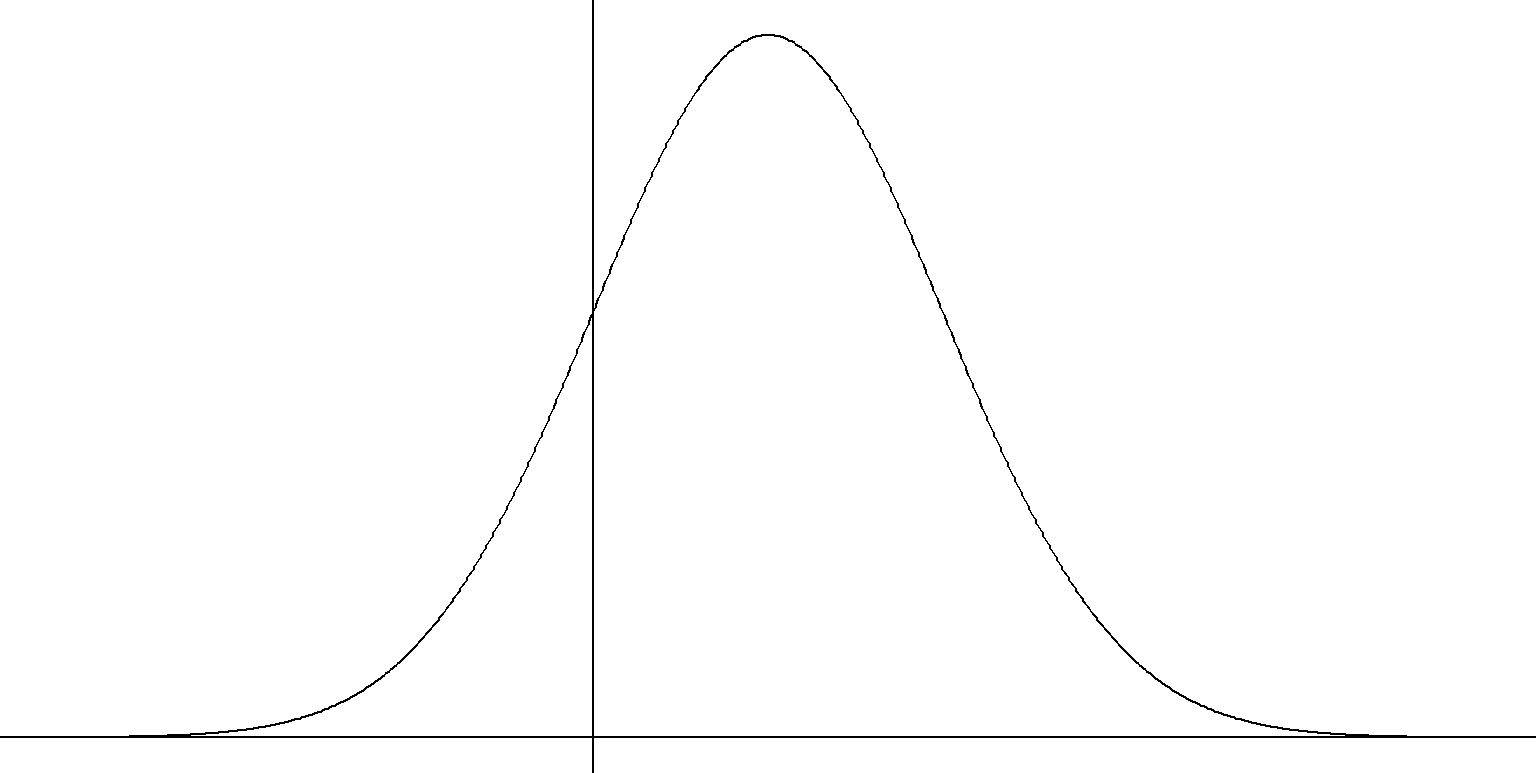
\includegraphics[width = 10cm]{img/im4_1.png}
    \caption{}
    \label{im4_1}
\end{figure}

给定置信水平$\alpha$,拒绝域为$W^+\geq c$,其中
\begin{equation*}
    c=\inf\{c^*:P(W^+\geqslant c^+)\leqslant\alpha\}
\end{equation*}

2、备择假设$H_1:\theta<0$,拒绝域为$W^+\leq d$,其中
\begin{equation*}
    d=\sup\{d^{*}:P(\begin{array}{c}W^{+}\leq d^{*}\\\end{array})\leq\alpha\}
\end{equation*}

3、备择假设$H_1:\neq 0$,拒绝域为$W^+\geq c$或$W^+\leq d$,其中
\begin{equation*}
    c=\inf\{c^*:P(W^+\geqslant c^*)\leqslant\alpha/2\},
    d=\sup\{d^*:P(W^+\leqslant d^*)\leqslant\alpha/2\}.
\end{equation*}

\section{符号秩和检验统计量$W^+$的性质}
\subsection{概率分布}
\begin{proposition}
    令$S=\sum_{i*1}^niu_i$,则在总体关于原点对称时,$W^+$和$S$同分布,
    即$W^+\overset{d}{\operatorname*{=}}S$。
\end{proposition}
\textbf{注:}总体X的分布关于原点对称时,$u_1,u_2,...,u_n$相互独立同分布,且$P(u_i=0)=P(u_i=1) = \frac12
    ,i=1,2,..,n $。故$S=\sum_{i=1}^{n}iu_i$为离散型分布,它的取值范围为$0,1,..,\frac{n(n+1)}2$,并且
\begin{equation}
    P(S=d)=P(\sum_{i=1}^niu_i=d)=\frac{t_n(d)}{2^n},d=0,1,2,\cdots,\frac{n(n+1)}2
\end{equation}
其中$t_n(d)$表示从$1,2,..,n$中任取若干个数,其和恰为d的取法数量(其中$t_n(d)=t_n(\frac{n(n+1)}{2}-d)$)。

\subsection{$W^+$分布的对称性}
\begin{proposition}
    在总体的分布关于原点0对称时,$W^+$服从对称分布,对称中心为$0,1,...,\frac{n(n+1)}2$的中点$\frac{n(n+1)}4$
\end{proposition}
\textbf{注:}当$n\leq 30$时,可查表得到符号秩和检验临界值$c_\alpha$,使$P(W^+\geq c_\alpha)=\alpha$,
故当$d=\frac{n(n+1)}2-c_\alpha$时,$P(W^+\leq d_\alpha)=\alpha$。

\section{符号秩和检验统计量$W^+$的渐进正态性}
\subsection{期望与方差}
$H_0$成立时,$W^+\overset{d}{\operatorname*{=}}S=\sum_{i=1}^{n}iu_i$,
$u_i\sim\begin{pmatrix}
        0       & 1       \\
        \frac12 & \frac12
    \end{pmatrix}$。
再根据$E(u_i)=\frac12,D(u_i)=\frac14$,求得S的期望与方差为
\begin{equation}
    \begin{aligned}
        E(S) & =\frac12\sum_{i=1}^ni=\frac{n\left(n+1\right)}4,                       \\
        D(S) & =\frac14\sum_{i=1}^ni^2=\frac{n\left(n+1\right)\left(2n+1\right)}{24}.
    \end{aligned}
\end{equation}
由于$W^+$与S有相同的分布,所以我们求得了$W^+$的均值与方差。
\begin{proposition}
    在总体分布关于原点0对称时,
    \begin{equation}
        \begin{aligned}
            E(W^+) & =\frac{n\left(n+1\right)}4,                     \\
            D(W^+) & =\frac{n\left(n+1\right)\left(2n+1\right)}{24}.
        \end{aligned}
    \end{equation}
\end{proposition}

\subsection{$W^+$渐进正态性}
由liapunov中心极限定理知S渐进服从正态分布,而$W^+$与S有相同的分布,
所以$W^+$也有渐进正态性。

\begin{proposition}
    如果总体的分布关于原点0对称,则在样本容量n趋于无穷大时,$W^+$也有渐进正态性,即
    \begin{equation}
        \frac{W^+-E\left(W^+\right)}{\sqrt{D\left(W^+\right)}}
        =\frac{W^+-n\left(n+1\right)/4}{\sqrt{n\left(n+1\right)\left(2n+1\right)/24}}
        \xrightarrow{L}N(0,1)
    \end{equation}
    该渐进正态性简记为
    \begin{equation}
        W^+\dot{\sim}N(\frac{n(n+1)}{4},\frac{n(n+1)(2n+1)}{24})
    \end{equation}
\end{proposition}

\section{平均秩法}
\subsection{定义}
\begin{definition}
    设$x_1,x_2,...,x_n$为取自总体X的样本,其中相等的$x_i$组成一个结,结中$x_i$的个数称为该结的结长$\tau(\geq 2)$
    ,结的个数记为$g$。
\end{definition}
秩的定义方式:随机秩,平均秩。

\subsection{性质}
\begin{proposition}
    若总体X的分布关于原点对称,有结数据取平均秩,则
    \begin{equation}
        \begin{aligned}
            E(W^+)             & =\frac{n(\left.n+1\right)}4,                                                            \\
            D(\left.W^+\right) & =n(\left.n+1\right)(\left(2n+1\right)/24-\sum_{j=1}^{g}\left(\tau_j^3-\tau_j\right)/48.
        \end{aligned}
    \end{equation}
\end{proposition}
\textbf{注:}有结数据取平均秩,$W^+$依旧服从渐进正态分布。

\section{对称中心的点估计}
\textbf{1、}样本的均值估计对称中心$\theta$。

\textbf{2、}样本的中位数估计对称中心$\theta$。

\textbf{3、}样本的切尾均值估计对称中心$\theta$。

\textbf{4、}Winsort化样本的均值估计对称中心$\theta$。
\begin{definition}
    设$x_1,x_2,...,x_n$的次序统计量为$x_{(1)},x_{(2)},...,x_{(n)}$,称
    \begin{equation}
        W_{nk} = \frac1n(\sum_{i = k+1}^{n-k}x_{(1)} + kx_{(k+1)} + kx_{(n-k)})
    \end{equation}
    为对称中心的Winsort化均值估计。
\end{definition}
\textbf{注:}Winsort化均值估计为切尾均值的一个修正,它加重了端头值在估计中的权重。

\textbf{5、}Hodges Lehmann(H-L)估计

H-L估计对称中心步骤如下:
\begin{enumerate}[(i)]
    \item 先构造统计量$T = T(x_1,x_2,...,x_n)$满足一下性质:
          \begin{itemize}
              \item $\theta = 0$时,T的分布关于某点c对称,且与x分布函数$F(x)$。
              \item 任意$x_1,x_2,...,x_n\in R$时,$T(x_1+\theta,x_2+\theta,...,x_n+\theta)$关于$\theta$非降。
          \end{itemize}
    \item 定义:
          \begin{equation}
              \begin{aligned}
                  \hat{\theta}_1 = \mathrm{sup}\{a:T(x_1-a,x_2-a,...,x_n-a)>c\} \\
                  \hat{\theta}_2 = \mathrm{sup}\{a:T(x_1-a,x_2-a,...,x_n-a)<c\}
              \end{aligned}
          \end{equation}
          一般有$\hat{\theta}_1 \leq\hat{\theta}_2$。
    \item 令$\theta = \frac{\hat{\theta}_1+\hat{\theta}_2}2$作为对称中心$\theta$的估计。
\end{enumerate}
常用对称中心H-L估计量如下:
\begin{enumerate}[(1)]
    \item 当T统计量为$T = \frac{\sqrt{n}\bar{x}}{S}$时,$\hat{\theta} = \bar{x}$;
    \item 当T统计量为$T = S^+= \{x_i>0,i = 1,2,..,n\}$时,$\hat{\theta} = m_n(\text{中位数})$;
    \item 当T统计量为$T = W^+$时,将$\{\frac{x_i+x_j}{2},1\leq i\leq j\leq n\}$,共有$N = \frac{n(n+1)}{2}$
          个值,从小到大排序为$W_{(1)}^+\leq W_{(2)}^+\leq...\leq W_{(N)}^+$,则称对称中心$\theta$的H-L估计为
          $\{\frac{x_i+x_j}{2},1\leq i\leq j\leq n\}$的中位数。
\end{enumerate}

\chapter{两样本问题}
\section{Mood中位数检验法($2\times 2$列联表检验法)}
\subsection{Mood中位数检验法}
样本$x_1,...,x_m$和$y_1,...,y_n$分别来自相互独立的连续型总体X和Y,分别记其中位数
为$me_x,me_y$。($H_0:me_x = me_y$)

首先将样本$x_1,..,x_m$和$y_1,...,y_n$合在一起,并从小到大排列,计算混合样本中位数$m_n$,
得四格表
\begin{table}[hp]
    \centering
    \caption{}
    \begin{tabular}{c|c|c|c}
              & $\leq m_n$ & $\geq m_n$ & 合计     \\
        \hline
        X样本 & $N_{11}$   & $N_{12}$   & $N_{1+}$ \\
        \hline
        Y样本 & $N_{21}$   & $N_{22}$   & $N_{2+}$ \\
        \hline
              & $N_{+1}$   & $N_{+2}$   & $N$      \\
    \end{tabular}
\end{table}

\textbf{1、}备择假设为$H_1:me_x> me_y$

当$N_{11}$较小时,拒绝$H_0$,检验$p$值为
$$
    \sum_{k\leq N_{11}}P(k,N_{1+},N_{+1},N)
$$

\textbf{2、}备择假设为$H_1:me_x< me_y$

当$N_{11}$较大时,拒绝$H_0$,检验$p$值为
$$
    \sum_{k\geq N_{11}}P(k,N_{1+},N_{+1},N)
$$

其中$P(k,N_{1+},N_{+1},N) = \frac{{N_{+1} \choose N_{11}}{N_{+2} \choose N_{12}}}
    {{N \choose N_{1+}}}$。

\subsection{大样本情形}
当样本容量较大时,超几何分布可以近似服从正态分布,过程与上一章大样本情形类似,此处过程省去。

\section{Wilcoxon秩和检验法}
\subsection{秩}
\begin{definition}
    设$x_1,...,x_{N}$是取自总体X的简单随机样本,我们定义$x_{i}$的秩$R_i$为
    \begin{equation}
        R_i = \sum_{j=1}^{N}I_{(x_{j}\leq{x_{i}})}
    \end{equation}
\end{definition}

\begin{definition}
    设$x_1,...,x_{N}$是取自总体X的简单随机样本,$R_i$为$x_i$的秩,则$R = (R_1,R_2,...,R_N)$或部分分量$(R_1,R_2,...,R_m)(1\leq m \leq N)$或由$R$构成的统计量统称为秩统计量。
\end{definition}

\begin{proposition}
    对于简单随机样本$x_1,...,x_{N}$,秩统计量$R = (R_1,R_2,...,R_N)$等可能的取$(1,2,...,N)$的任意$N!$个排列之一,且$R$是由在$(1,2,...,N)$的所有可能的排列组成的空间$R$上的均匀分布,即
    \begin{equation}
        P(R = (r_1,r_2,...,r_N)) = \frac{1}{N!}
    \end{equation}
\end{proposition}
\textbf{注:}对于简单随机样本,R的边缘分布也是均匀分布,如
\begin{equation}
    \begin{aligned}
        & P(R_i = r) = \frac1N, r = 1,2,...,N \\
        & P(R_i=r_1,R_j=r_2) = \frac1{N(N-1)}, r_1(\text{或}r_2) = 1,2,...,N, r_1\neq r_2
    \end{aligned}
\end{equation}

\begin{theorem}
    对$\forall~i = 1,2,...,N$,有
    \begin{equation}
        E(R_i)=\frac{N+1}2,~V(R_i)=\frac{N^2 -1}{12}
    \end{equation}
\end{theorem}

\begin{theorem}
    对$\forall~i \neq j$,有
    \begin{equation}
        \mathrm{Cov}(R_i,R_j) = -\frac{N+1}{12}
    \end{equation}
\end{theorem}

\subsection{Wilcoxon秩和检验统计量的性质}
设两样本$x_1,x_2,...,x_{m}$和$y_1,y_2,...,y_n(m \geq n)$,样本容量$N = m + n$。

Wilcoxon秩和检验原假设$H_0:X$与$Y$同分布。$H_0$成立时,
$$
    P(R_1=r_1,R_2=r_2,\cdots,R_n=r_n)=\frac1{N(N-1)\cdots(N-n+1)}
$$
其中$(r_1,r_2,...,r_n)$是从$1,2,...,N$中取出的$n$个数的一个排列。

记Y样本$y_1,y_2,...,y_n$的秩和为$W_y$,即
\begin{equation}
    W_y = \sum_{j=1}^{n}R_{j}
\end{equation}

\textbf{1、概率分布}

$W_y$服从离散型分布,最小值为$1+2+\cdots+n=\frac{n(n+1)}{2}$,最大值为$(m+1)+(m+2)+\cdots+(m+n)=mn+\frac{n(n+1)}{2}$。

\begin{proposition}
    当$H_0$成立时,
    \begin{equation}
        \begin{aligned}
            P(W_y = d) &= P(\sum_{j=1}^{n}R_{j} = d) =  \frac{t_{m,n}(d)}{C_N^n}\\
            P(W_y \leq d) &= P(\sum_{j=1}^{n}R_{j} \leq d) =  \frac{\sum_{j\leq d}t_{m,n}(j)}{C_N^n}\\
        \end{aligned}
    \end{equation}
    其中$t_{m,n}(d)$表示从$1,2,...,N$中任取n个数,其和恰为d的取法总数。
\end{proposition}

\textbf{2、对称性}

假设从$1,2,...,N$中任取n个数为$a_1,a_2,...,a_n$,其和为d,若令$b_i = N+1-a_i$,则$1\leq b_i \leq N,~i = 1,2,...,n$,其和为$n(N+1)-d$,则$t_{m,n}(d) = t_{m,n}(n(N+1)-d)$。

故有以下结论:
\begin{equation}
    \begin{aligned}
        P(W_y=d)&=P(W_y=n(N+1)-d)\\
        P(W_y\leqslant d)&=P(W_y\geqslant n(N+1)-d)
    \end{aligned}
\end{equation}
其中$d = \frac{n(n+1)}{2},1+\frac{n(n+1)}{2},...,mn+\frac{n(n+1)}{2}$。

特别地,我们可以推出
\begin{equation}
    \begin{aligned}
        P(W_y=n(N+1)/2-d)&=P(W_y=n(N+1)/2+d)\\
        P(W_y\leqslant n(N+1)/2-d)&=P(W_y\geqslant n(N+1)/2+d)
    \end{aligned}
\end{equation}

\begin{proposition}
    当$H_0$成立时,$W_y$服从对称分布,对称中心为$\frac{n(N+1)}{2}$。
\end{proposition}

\textbf{3、$W_y$的期望和方差}
\begin{proposition}
    当$H_0$成立时,
    \begin{equation}
        \begin{aligned}
            E(W_y) &= \frac{n(N+1)}{2} \\
            D(W_y) &= \frac{mn(N+1)}{12}
        \end{aligned}
    \end{equation}
\end{proposition}

\textbf{4、渐进正态性}
\begin{proposition}
    $H_0$成立时,若$min\{m,n\}\rightarrow \infty$,且$\frac{m}N \rightarrow \lambda \in (0,1),~\lambda$为常数,则
    \begin{equation}
        \frac{W_y-E(W_y)}{\sqrt{D(W_y)}}=\frac{W_y-n\left(N+1\right)/2}{\sqrt{mn\left(N+1\right)/12}}\xrightarrow{L}N(0,1).
    \end{equation}
\end{proposition}

\subsection{Wilcoxon秩和检验的备择假设}
原假设$H_0:$X和Y同分布。而Wilcoxon秩和检验的备择假设有四种定量描述方法。

\textbf{1}、备择假设:$H_1:P(X>Y)>\frac12;P(X>Y)<\frac12;P(X>Y)\neq \frac12$。

\textbf{2}、设总体X和Y的分布函数、密度函数为$F(x),G(x),f(x),g(x)$,则$H_1:F < G; F > G; F\neq G$。
\begin{theorem}
    设总体X和Y相互独立,$\forall c\in \mathbb{R} $,都有$F(c)<G(c)$,则$P(X>Y)>\frac12$。
\end{theorem}

\textbf{3}、若X+a和Y同分布,则a为位置参数,$H_1:a>0;a<0;a\neq 0$。
\begin{theorem}
    X+a与Y同分布,当且仅当$\forall c\in \mathbb{R}$,有$G(c)= F(c-a)$。
\end{theorem}

\textbf{4}、$H_1:me_x > me_y; me_x < me_y; me_x \neq me_y$。
\begin{theorem}
    \begin{enumerate}[(1)]
        \item $\forall c \in \mathbb{R}$,都有$F(c) < G(c)$,则$me_x > me_y$。
        \item 假设$X+a\overset{d}{=}Y$或$\forall c \in \mathbb{R}$,都有$F(c-a) = G(c)$,则$me_x+a = me_y$。
    \end{enumerate}
\end{theorem}

\textbf{注:}以上四种备择假设的关系:$3 \rightarrow 2 \rightarrow 1,~ 3 \rightarrow 2 \rightarrow 4$。

\subsection{Wilcoxon秩和检验的平均秩}
$W_y = \sum_{i = 1}^{n}a(R_i)$,其中$a(r),r = 1,2,...,n$为计分函数。结长为1时,$a(r) = r$;结长大于1时,$a(r)$为结长的平均秩。

\textbf{1、计分函数$a(R_i)$的性质}
\begin{equation}
    \begin{gathered}
    E(a(R_{i}))=\bar{a}  \\
    D(a(R_i))=\frac{1}{N}\sum_{i=1}^{N}(a(i)-\overline{a})^2 \\
    \mathrm{Cov}\left(a(R_{i}),a(R_{j})\right)=-\frac{1}{N(N-1)}\sum_{i=1}^{N}(a(i)-\overline{a})^{2} 
    \end{gathered}
\end{equation}
其中$\bar{a} = \frac{\sum_{i=1}^N a(i)}N$。

\begin{theorem}
    在X和Y同分布时,有
    \begin{equation}
        \begin{aligned}
            E(\sum_{i=1}^na(R_i))&=n\overline{a}\\
            D(\sum_{i=1}^na(R_i))&=\frac{nm}{N(N-1)}\sum_{i=1}^n(a(i)-\overline{a})^2
        \end{aligned}
    \end{equation}
\end{theorem}

\textbf{2、$W_y$的数字特征及渐进分布}
\begin{equation}
    \begin{gathered}
    E(\alpha(R_i))=\alpha=\frac{n(N+1)}{2} \\
    D(\alpha(R_i))=\frac{nm(N+1)}{12}-\frac{nm}{12N(N-1)}\sum_{j=1}^{g}(\tau_j^3-\tau_j)
    \end{gathered}
\end{equation}

\subsection{位置参数差的检验与估计}
若$\exists a$,对$\forall ~ c \in \mathbb{R}$,都有$G(c) = F(c-a)$,则X+a与Y同分布。

\textbf{1、位置参数差的检验}
\begin{center}
    $H_0:a = \eta $ vs $H_1:a < \eta; a \neq \eta; a > \eta$
\end{center}
若$H_0$成立,则$X+\eta$与Y同分布。

\textbf{2、位置参数差的估计}
\begin{enumerate}[(1)]
    \item 点估计:
    \begin{enumerate}[(a)]
        \item 样本均值差估计位置参数差:$\hat{a} = \bar{y}-\bar{x}$;
        \item 样本中位数差估计位置参数差:$\hat{a} = me_{y}-me_{x}$;
        \item H-L估计:$\hat{a} = me(Y-X)$,即$\{y_j - x_i,i = 1,...,m,j = 1,...,n\}$的中位数。
    \end{enumerate}
    \item 区间估计。
\end{enumerate}

\section{Mann-Whitney U检验}
\subsection{U统计量}
\textbf{1、单样本U统计量}
\begin{definition}
    设$x_1,x_2,...,x_n$为取自总体X的样本,h为m元函数$(m\leq n)$,若$h(x_1,x_2,...,x_m)$为总体分布参数$\theta$的无偏估计,即
    \begin{equation}
        E(h(x_1,x_2,...,x_m))=\theta
    \end{equation}
    则称$U_n = U_n(x_1,x_2,...,x_n) = \frac1{A_n^m}\sum_{1\leq i_1\neq i_2\neq\ldots\neq i_m\leq n}h(x_{i_1},\ldots x_{i_m})$为U统计量,或称其是以函数h为核的基于样本$x_1,x_2,...,x_n$的参数$\theta$的U统计量。
\end{definition}
\textbf{注:}
\begin{enumerate}[(i)]
    \item U统计量是$\theta$的无偏估计,即$E(U_n) = \theta$;
    \item 若核函数h为对称核函数,即任一$(1,2,...,m)$的排列$\alpha_{1},\alpha_{2},...,\alpha_{m}$,有
    $h(x_{\alpha_1},x_{\alpha_2},...,x_{\alpha_m})=h(x_1,x_2,...,x_m)$,则U统计量可以简写为:
    \begin{equation}
        U_n = \frac1{C_n^m}\sum_{1\leq i_1\neq i_2\neq\ldots\neq i_m\leq n}h(x_{i_1},\ldots x_{i_m})
    \end{equation}
    \item 若核函数h不是对称核函数,可以构造等价的对称核函数
    \begin{equation}
        h^*(x_1,\ldots,x_m)=\frac1{m!}\sum_{1\leq i_1\neq i_2\neq\ldots\neq i_m\leq m}h(x_{i_1},\ldots,x_{i_m})
    \end{equation}
    其中$(i_1,i_2,...,i_m)$为$(1,2,...,m)$的任意排列。
\end{enumerate}

\textbf{2、两样本U统计量}
\begin{definition}
    设$x_1,x_2,...,x_m$和$y_1,y_2,...,y_n$分别为取自分布为$F(x)$的总体X和分布为$G(y)$的总体Y的样本,h为$m_1+m_2$元函数。
    若$h(x_1,x_2,...,x_{m_1},y_1,y_2,...,y_{m_2})$为总体分布参数$\theta$的无偏估计,即$E(h(x_1,x_2,...,x_{m_1},y_1,y_2,...,y_{m_2}))=\theta(F,G)$,
    则以h为核基于两样本$(x_1,x_2,...,x_m,y_1,y_2,...,y_n)$的参数$\theta$的U统计量为
    \begin{equation}
        U_{mn} = \frac1{A_m^{m_1}A_n^{{m}_2}}\sum_{(1\leq i_1\neq\ldots\neq i_{m_1}\leq m)}\sum_{(1\leq j_1\neq\ldots\neq j_{m_2}\leq n)}h(x_{i_1},\ldots,x_{i_{m_1}},y_{j_1},\ldots,y_{j_{m_2}})
    \end{equation}
\end{definition}
\textbf{注:}
\begin{enumerate}
    \item U统计量是$\theta$的无偏估计,即$E(U_{mn}) = \theta$;
    \item 若核函数h为对称核函数,即任一$(1,2,...,m_1)$的排列$(\alpha_{1},\alpha_{2},...,\alpha_{m_1})$和$(1,2,...,m_2)$的排列$(\beta_{1},\beta_{2},...,\beta_{m_2})$,有
    \begin{equation}
        U_{mn} = \frac1{C_m^{m_1}C_n^{{m}_2}}\sum_{(1\leq i_1\neq\ldots\neq i_{m_1}\leq m)}\sum_{(1\leq j_1\neq\ldots\neq j_{m_2}\leq n)}h(x_{i_1},\ldots,x_{i_{m_1}},y_{j_1},\ldots,y_{j_{m_2}})
    \end{equation}
    \item 若核函数h不是对称核函数,构造等价的对称核函数
    \begin{equation}
        h^*(x_1,\ldots,x_{m_1},y_1,\ldots,y_{m_2})=\frac1{m_1!m_2!}\sum_{(1\leq i_1\neq\ldots\neq i_{m_1}\leq m_1)}\sum_{(1\leq j_1\neq\ldots\neq j_{m_2}\leq m_2)}h(x_{i_1},\ldots,x_{i_{m_1}},y_{j_1},\ldots,y_{j_{m_2}})
    \end{equation}
\end{enumerate}

\subsection{Mann-Whitney U统计量$(W_{xy})$和Wilcoxon秩和检验统计量$(W_y)$}

\textbf{1、Mann-Whitney U统计量}
\begin{equation}
    \Phi(x_{i},y_{j})=\begin{cases}{1,\quad x_{i}-y_{j}<0}\\{0,\quad\text{其他}}\end{cases}
\end{equation}
则$W_{xy} = \sum_{i = 1}^m\sum_{j = 1}^n \Phi(x_i,y_j)$。

\textbf{2、$W_{xy}$和$W_y$}
\begin{theorem}
    $W_{xy}$和$W_{y}$仅相差一个常数,即:$W_{xy} = W_y - \frac{n(n+1)}2;W_{yx} = W_x - \frac{m(m+1)}2$。
\end{theorem}
\textbf{注:}“用Mann-Whitney U统计量作检验统计量”等价于“用Wilcoxon秩和统计量作检验统计量”。

\subsection{Mann-Whitney U统计量的性质}
\textbf{1、小样本情形}
\begin{proposition}
    若原假设$H_0$成立,则$W_{xy}$服从对称分布,分布中心为$\frac{mn}2$。由此可以推导出如下结论:
    \begin{equation*}
        \begin{gathered}
            P(W_y\leq d_{\alpha}) = \alpha \\
            P(W_{xy}\leq d_{\alpha} - \frac{n(n+1)}2)= \alpha \\
            P(W_{xy}\geq mn - d_{\alpha} + \frac{n(n+1)}2)= \alpha
        \end{gathered}
    \end{equation*}
\end{proposition}

\textbf{2、大样本情形}
\begin{proposition}
    若原假设$H_0$成立,则有
    \begin{equation}
        \begin{aligned}
            \mathrm{EW_{xy}=EW_y-n(n+1)/2=mn/2}\\
            \mathrm{DW_{xy}=DW_y=mn(N+1)/12}
        \end{aligned}
    \end{equation}
    且若$min\{m,n\}\rightarrow \infty$,且$\frac{m}N \rightarrow \lambda \in (0,1),~\lambda$为常数,则$W_{xy}$有渐进正态性。
\end{proposition}

\section{两样本尺度参数的秩检验方法}

\subsection{尺度参数}
\textbf{1、定义}
\begin{definition}
    设总体X和Y的分布函数分别为$F(x)$和$G(x)$,若$F(0) = G(0) = \frac12$,且对任意实数c,有$G(c) = F(\frac{c}b)$,则称b为X与Y的尺度参数$(b >0)$。
\end{definition}

\begin{theorem}
    设总体X和Y的分布函数分别为$F(x)$和$G(x)$,若$F(0) = G(0) = \frac12$,且对任意实数c,都有$G(c) = F(\frac{c}b) \Longleftrightarrow $ bX与Y同分布。
\end{theorem}

\textbf{2、尺度参数b取值大小的意义}
\begin{enumerate}[(1)]
    \item $b > 1$,因为$p(Y>c)=p(bX>c)=p(X>c/b)$,则若$b>1$
    \begin{itemize}
        \item 当$c>0$时,$p(Y>c)>p(X>c)$;
        \item 当$c<0$时,$p(Y<c)>p(X<c)$。
    \end{itemize}
    \item $b<1$,分析与上面的类似。
\end{enumerate}

\textbf{3、}

若b为X与Y的尺度参数,则有
\begin{equation}
    {\sigma_y}^2={\mathrm{b}}^2{\sigma_x}^2,{\mathrm{IQR}}_y={\mathrm{b}}({\mathrm{IQR}}_x)
\end{equation}

\subsection{尺度参数的检验问题}
\begin{center}
    $H_0: b = 1 ~vs~ H_1: b > 1; b < 1; b \neq 1$ 
\end{center}
\begin{definition}
    积分函数$\alpha(r),r = 1,2,...,n$,$y_i$的秩为$R_i$时,$y_i$的得分为$\alpha(R_i)$。
\end{definition}

\textbf{1、Mood检验}

取$\alpha(r) = (r - \frac{N+1}2)^2,r = 1,2,...,N$,此时$\alpha(r)$为单谷函数,记$M_y = \sum_{i = 1}^n\alpha(R_i)$。则当$H_0$成立时,有
\begin{equation}
    E(M_y) = \frac{n(N^2-1)}{12}, ~ D(M_y) = \frac{nm(N+1)(N^2-4)}{180}
\end{equation}
且若$min{m,n} \rightarrow \infty$,且$\frac{m}N \rightarrow \lambda \in (0,1),~\lambda$为常数,则$M_y$有渐进正态性。

\textbf{2、Siegal-Turkey检验}

\textbf{3、Ansari-Bradley检验}

取$\alpha(r)$为单峰函数,令$\alpha(r) = \frac{N+1}2 - \|r - \frac{N+1}2\|,r = 1,2,...,N$,记$A = \sum_{i = 1}^N\alpha(R_i)$。

\textbf{4、Klotz检验}

记标准正态分布的分布函数为$\Phi(x)$,取$\Phi(x)$的反函数$\Phi^{-1}(x)$,取$\alpha(r) = [\Phi^{-1}(\frac{r}{N+1})]^2,r = 1,2,...,N$,则$\alpha(r)$为单谷函数,记$K_y = \sum_{i = 1}^N\alpha(R_i)$。

\chapter{多样本问题}
\section{Kruskal-Wallis检验法}
\subsection{Kruskal-Wallis检验}
\textbf{1、H的分析}

\begin{itemize}
    \item 组间平方和:$SSB = \sum_{j = 1}^kn_j (\bar{x}_j - \bar{x})^2$;
    \item 组内平方和:$SSW = \sum_{i = 1}^k\sum_{j = 1}^{n_i}(x_{ij} - \bar{x}_i)^2$;
    \item 总平方和:$SST = \sum_{i = 1}^k\sum_{j = 1}^{n_i}(x_{ij} - \bar{x})^2$。
\end{itemize}









\begin{thebibliography}{3}
    \bibitem{ref1}孙山泽.非参数统计讲义.北京大学出版社
    \bibitem{ref2}陈希孺.非参数统计.中国科学技术大学出版社
    \bibitem{ref3}李裕奇.非参数统计方法.西南交通大学出版社
\end{thebibliography}

\end{document}